\documentclass[10pt,twocolumn]{article}

\usepackage[margin=0.8in,columnsep=0.28in]{geometry}
\usepackage{mathptmx}
\usepackage[T1]{fontenc}
\usepackage{microtype}
\usepackage{graphicx}
\usepackage{booktabs}
\usepackage{xcolor}
\usepackage{tikz}
\usetikzlibrary{arrows.meta,positioning}
\usepackage{caption}
\usepackage{enumitem}
\usepackage{fancyhdr}
\usepackage[colorlinks=true,linkcolor=blue!50!black,urlcolor=blue!50!black,citecolor=blue!50!black]{hyperref}

\definecolor{pfblue}{HTML}{1F6FEB}
\definecolor{pfpurple}{HTML}{8957E5}
\definecolor{pfgreen}{HTML}{2EA043}
\definecolor{pfgrey}{HTML}{57606A}

\pagestyle{fancy}
\fancyhf{}
\renewcommand{\headrulewidth}{0.3pt}
\fancyhead[L]{\small\color{pfgrey}SKZL-AI --- Paper Factory Position Paper}
\fancyhead[R]{\small\color{pfgrey}v1.0 --- 2026-10}
\fancyfoot[C]{\small\thepage}

\setlist{nosep,leftmargin=1.2em}
\captionsetup{font=small,labelfont={bf,color=pfblue}}

\title{\textbf{Paper Factory: Evidence-First Orchestration for\\[2pt] Agentic Research-Paper Production}\\[6pt]
\large Position Paper --- System v1.0.0}
\author{Furkan Sak{\i}zl{\i}\\
SKZL-AI\\
\texttt{https://github.com/SKZL-AI/paper-factory}}
\date{October 2026}

\begin{document}
\maketitle
\thispagestyle{fancy}

\begin{abstract}
\noindent
LLM-based agents can now draft scientific manuscripts end to end, but their
prose fluency systematically outpaces their evidentiary discipline: claims
appear without data, citations resolve to the wrong papers, self-verification
closes findings it never checked, and external editing tools mutate text
silently. We present \emph{Paper Factory}, a production system built on the
opposite premise. A deterministic orchestration core drives a research DAG
(P00--P37); LLM harnesses (Claude Code, Kimi, Codex, Pi, OpenCode,
LiteLLM-backed workers) are replaceable adapters, never authorities. Every
scientific claim must be bound to content-addressed evidence; sixteen global
closure invariants (U1--U16) fail closed; an independent verification kernel
(VeriHarness/HoH) checks work packages; and the two irreversible steps ---
final sign-off (P36) and external submission (P37) --- remain under human
authority by construction. We report evidence from operating the system on a
real research paper: 574 automated tests, a 16/16 closure-gate pass, an exact
SHA-256 artifact chain from raw data to the arXiv bundle, and 245
writing-assistant suggestions processed capture-only and fully dispositioned.
We argue that \emph{evidence-first orchestration}, not better prompting, is
the missing layer in agentic science.
\end{abstract}

\section*{Revision note (2026-10-05)}
This paper documents the \emph{v1.0.0} freeze; its design principles and
the evidence table remain the v1.0-era baseline, reported as of that
freeze. Later releases added, without changing the principles above: a
versioned verification-plane contract (v1.2), the Reproduction Plane and
a pure interchange export layer (v1.3), a Nextflow backend, CWL export,
and release artifact attestations (v1.4), and, with v2.0.0, a full
contract inventory with explicit stability guarantees. The current
architecture and contracts are maintained in
\texttt{docs/ARCHITECTURE.md} and \texttt{docs/CONTRACTS.md} of the
repository.

\section{Introduction: Prose Is Not Evidence}

Agentic LLM systems now search literature, run analyses, and write credible
manuscripts. What they do not do by default is \emph{prove} anything. Across
our own operation of multi-agent research pipelines we repeatedly observed
five failure modes:

\begin{enumerate}
\item \textbf{Unsupported claims.} Final-paper statements with no link to any
computed artifact.
\item \textbf{Citation misattribution.} References whose DOI resolves --- to
a \emph{different} paper than the one described.
\item \textbf{Vacuous remediation.} Review findings closed by generic
post-conditions (``no unsupported claims remain'') that never re-check the
concrete finding.
\item \textbf{Silent external edits.} Writing assistants (grammar/style
tools) rewriting text in ways that shift scientific meaning.
\item \textbf{Premature irreversible release.} Automation drifting toward
submission actions that should require a human.
\end{enumerate}

\noindent
These are not model-quality problems; they are \emph{systems} problems. A
more fluent model produces more fluent unsupported claims. Our position:
agentic science needs an orchestration layer in which \textbf{evidence is a
precondition of prose, verification is independent of generation, and closure
is a cryptographic-property-like invariant set --- not a summary an agent
writes about itself.}

\section{Design Principles}

Paper Factory implements seven principles:

\begin{description}[style=nextline]
\item[DP1 --- Deterministic core, probabilistic workers.]
The pipeline is a fixed DAG (P00--P37) executed by a deterministic core with
persistent, append-only state. LLM harnesses are interchangeable workers
behind a provider router; the backend model identity is recorded separately
from the harness name.
\item[DP2 --- Evidence before prose.]
Artifacts carry authority tiers T0--T4 (raw data and registries down to drafts
and chats). No empirical claim enters the paper without evidence linkage.
\item[DP3 --- Claim--evidence binding.]
Claims form a graph bound to concrete artifacts --- metrics, tables, analyses
--- each content-addressed by SHA-256. Numbers in prose are generated from
metrics via macros, never hand-typed.
\item[DP4 --- Independent verification.]
Work packages are verified by a separate kernel (VeriHarness/HoH:
plan\,\textrightarrow\,develop\,\textrightarrow\,independent
QA\,\textrightarrow\,receipts\,\textrightarrow\,accept/reject) integrated
through an adapter. The generator never grades itself.
\item[DP5 --- Fail-closed gates.]
Sixteen global closure invariants (U1--U16) audit claim support, citation
identity, number-to-metric binding, remediation integrity, and external-edit
reconciliation. Exit code 0 means \texttt{CLOSED} and nothing else;
insufficient evidence yields \texttt{DEGRADED}/\texttt{FAILED}, never a
fabricated pass.
\item[DP6 --- Human authority at irreversible steps.]
P36 is an explicit, receipt-bound human sign-off. P37 (external submission)
is never executed automatically.
\item[DP7 --- Append-only receipts.]
Every transition emits receipts; corrections amend history instead of
rewriting it. Reviews are adversarial by design (dual independent reviewers,
instructed to refute).
\end{description}

\begin{figure*}[t]
\centering
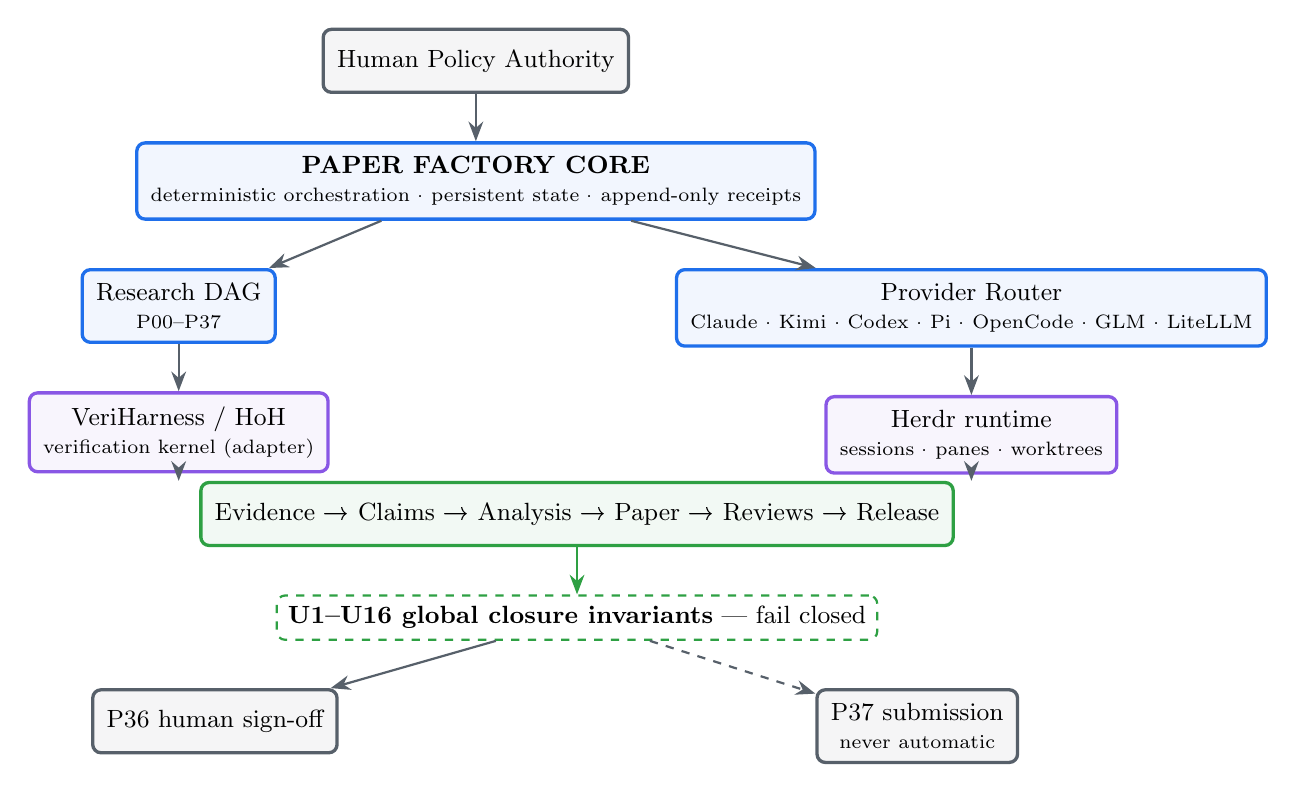
\begin{tikzpicture}[
  font=\small,
  box/.style={draw=#1, rounded corners=3pt, very thick, fill=#1!6, minimum height=8mm, inner sep=5pt, align=center},
  arr/.style={-{Stealth[length=2.5mm]}, thick, pfgrey},
]
% top-down spine
\node[box=pfgrey] (human) {Human Policy Authority};
\node[box=pfblue, below=6mm of human] (core) {\textbf{PAPER FACTORY CORE}\\[-1pt]
{\scriptsize deterministic orchestration · persistent state · append-only receipts}};
\node[box=pfblue, below left=6mm and -18mm of core] (dag) {Research DAG\\[-1pt]{\scriptsize P00–P37}};
\node[box=pfblue, below right=6mm and -18mm of core] (router) {Provider Router\\[-1pt]
{\scriptsize Claude · Kimi · Codex · Pi · OpenCode · GLM · LiteLLM}};
\node[box=pfpurple, below=6mm of dag] (vh) {VeriHarness / HoH\\[-1pt]{\scriptsize verification kernel (adapter)}};
\node[box=pfpurple, below=6mm of router] (herdr) {Herdr runtime\\[-1pt]{\scriptsize sessions · panes · worktrees}};
\path (vh) -- (herdr) coordinate[midway] (mid);
\node[box=pfgreen, below=6mm of mid] (chain) {Evidence \textrightarrow\ Claims \textrightarrow\ Analysis
\textrightarrow\ Paper \textrightarrow\ Reviews \textrightarrow\ Release};
\node[draw=pfgreen, dashed, thick, rounded corners=3pt, inner sep=4pt, below=6mm of chain, align=center] (gates)
  {\textbf{U1–U16 global closure invariants} --- fail closed};
\node[box=pfgrey, below left=6mm and -8mm of gates] (p36) {P36 human sign-off};
\node[box=pfgrey, below right=6mm and -8mm of gates] (p37) {P37 submission\\[-1pt]{\scriptsize never automatic}};

\draw[arr] (human) -- (core);
\draw[arr] (core) -- (dag);
\draw[arr] (core) -- (router);
\draw[arr] (dag) -- (vh);
\draw[arr] (router) -- (herdr);
\draw[arr] (vh.south) -- (chain.north -| vh.south);
\draw[arr] (herdr.south) -- (chain.north -| herdr.south);
\draw[arr, pfgreen] (chain) -- (gates);
\draw[arr] (gates) -- (p36);
\draw[arr, dashed] (gates) -- (p37);
\end{tikzpicture}
\caption{Paper Factory architecture. The deterministic core owns \emph{what}
must happen; the verification kernel owns \emph{whether} it happened; the
runtime owns sessions and isolation; the human owns irreversible steps.}
\label{fig:arch}
\end{figure*}

\section{Architecture}

Figure~\ref{fig:arch} shows the layering. The core (this system) is a Python
CLI --- \texttt{paper-factory complete} runs from a plain shell with no
interactive assistant involved. State lives in SQLite plus immutable
JSON/JSONL/YAML artifacts; every node of the DAG reads and writes
content-addressed evidence.

Three boundaries are load-bearing. (i)~\emph{Adapter boundary:} harnesses are
workers; swapping Claude Code for Kimi changes labor, not truth.
(ii)~\emph{Verification boundary:} VeriHarness/HoH decides accept/reject on
receipts; Paper Factory cannot override a rejection.
(iii)~\emph{Authority boundary:} a provenance firewall decides which process
may write protected paths (e.g.\ final prose); unknown backends are denied by
default, and external edits (e.g.\ a writing assistant operating on a DOCX)
are reconciled against the frozen canonical manuscript via claim, number,
citation, and math diffs before they can influence the release.

\section{Evidence from Operation}

Paper Factory v1.0.0 was frozen only after a real end-to-end pilot: a
mass-invariance research paper taken from draft-assisted intake through
analysis, citation verification, external writing-assistant review (Microsoft
Word + Paperpal, driven ownership-scoped and capture-only), adversarial dual
review, and arXiv-bundle packaging. Table~\ref{tab:evidence} summarizes.

\begin{table}[t]
\centering\small
\caption{Operational evidence at the v1.0.0 freeze.}
\label{tab:evidence}
\begin{tabular}{@{}p{0.60\columnwidth}r@{}}
\toprule
\textbf{Measure} & \textbf{Result} \\
\midrule
Automated tests & 574 passed, 2 skips \\
Pipeline nodes P21--P36 & all PASS \\
Closure invariants U1--U16 & 16/16 PASS \\
Node summary & 33 / 4 / 0 \\
Citations verified & 21/21 \\
Writing-assistant suggestions (unique) & 245 \\
\quad applied under semantic guards & 75 \\
\quad rejected with evidence & 124 \\
\quad not applicable & 46 \\
\quad undispositioned & 0 \\
Artifact hash chain end-to-end & MATCH \\
P37 external submission & NOT RUN \\
\bottomrule
\end{tabular}
\end{table}

Two observations matter more than the pass counts. First, hardening
\emph{increased} honest failures during development: making remediation
finding-specific (killing vacuous resolution) and binding numbers to named
metrics surfaced real defects that summary-level checks had hidden. A system
that never fails is not strict; it is unaudited. Second, all 124 rejected
writing-assistant suggestions were rejected \emph{with evidence}, and none
of the 245 unique suggestions touched the manuscript silently --- external-edit reconciliation (U16) is a
gate, not a diff nobody reads.

\subsection{The Closure Invariants}

For concreteness, the sixteen invariants every run must satisfy verbatim:

\begin{enumerate}[label=\textbf{U\arabic*.},leftmargin=2.6em]
\item Every primary claim has evidence.
\item Every scientific number matches generated source.
\item Figures/tables match their manifests.
\item Citations resolve and support the contextual claim.
\item No unresolved CRITICAL/MAJOR review finding.
\item Reviewed manuscript $=$ release manuscript.
\item Code/data commits match manifests.
\item No secrets or private transcripts enter the release.
\item Writing-assistant state is PASS or explicit HUMAN\_REQUIRED.
\item The clean bundle independently rebuilds.
\item Final-prose files have allowed origin receipts.
\item Forbidden model families did not modify protected prose.
\item Backend identity is known for final writer invocations.
\item Marking status is reported honestly.
\item Reviewer replacement prose is not silently copied.
\item External writing-assistant edits underwent semantic reconciliation.
\end{enumerate}

None of these is a prompt. Each is an executable check over artifacts,
receipts, and hashes, evaluated by the core at closure time --- an agent
cannot argue its way past them.

\section{Limitations and Open Problems}

We are deliberately not claiming generality. (i)~Evidence comes from one real
pilot family plus synthetic suites; broader intake modes (data-only,
code-only) need more pilots. (ii)~Semantic-diff artifacts are partially
assertion-level markers, not deep proofs. (iii)~External-tool automation
(e.g.\ a writing assistant's web pane) is inherently UI-fragile; we mitigate
with capture-only semantics and ownership-scoped process control, but drift
remains an operational risk. (iv)~The verification kernel and runtime have
their own maturity limits; Paper Factory records these honestly as
\texttt{DEGRADED} rather than hiding them. (v)~Exit-code discipline and
closure invariants resist, but cannot eliminate, adversarial or confused
\emph{human} overrides; durable human decisions are therefore
append-only and collision-hardened, yet still human.

\section{Related Work}

The system builds on established infrastructure rather than replacing it:
large language models as workers~\cite{vaswani2017attention}; community
scholarly-metadata registries for citation identity
(Crossref~\cite{hendricks2020crossref}, OpenAlex~\cite{priem2022openalex});
and W3C PROV as the conceptual basis for artifact
provenance~\cite{lebo2013prov}. VeriHarness/HoH contributes the
harness-of-harnesses verification model with receipts and pre-registered
gates~\cite{skzl2026veriharness}. Relative to agentic writing frameworks,
Paper Factory's distinction is negative as much as positive: it is designed
around everything an agent must \emph{not} be trusted to do --- grade itself,
close findings vacuously, edit prose silently, or submit irreversibly.

\section{Conclusion and Call to Action}

Agentic science will be believed exactly to the extent that its artifacts are
auditable. We offer Paper Factory as one concrete, operating answer:
deterministic orchestration, evidence-bound claims, independent verification,
fail-closed closure invariants, and humans at the irreversible steps. The
system, its test suite, its freeze evidence, and its honest list of
limitations are public. We invite the community to attack the invariants ---
that is what they are for.

\begin{thebibliography}{9}\small

\bibitem{vaswani2017attention}
A.~Vaswani, N.~Shazeer, N.~Parmar, J.~Uszkoreit, L.~Jones, A.~N. Gomez,
{\L}.~Kaiser, I.~Polosukhin.
\newblock Attention is all you need.
\newblock \emph{NeurIPS}, 2017. arXiv:1706.03762.

\bibitem{hendricks2020crossref}
G.~Hendricks, D.~Tkaczyk, J.~Lin, P.~Feeney.
\newblock Crossref: The sustainable source of community-owned scholarly
metadata.
\newblock \emph{Quantitative Science Studies}, 1(1):414--427, 2020.

\bibitem{priem2022openalex}
J.~Priem, H.~Piwowar, R.~Orr.
\newblock OpenAlex: A fully-open index of scholarly works, authors, venues,
institutions, and concepts.
\newblock \emph{26th International Conference on Science, Technology and
Innovation Indicators}, 2022.

\bibitem{lebo2013prov}
T.~Lebo, S.~Sahoo, D.~McGuinness (eds.).
\newblock PROV-O: The PROV ontology.
\newblock \emph{W3C Recommendation}, 2013.

\bibitem{skzl2026veriharness}
SKZL-AI.
\newblock VeriHarness: An evidence-bound harness-of-harnesses for verifiable
long-horizon agent development.
\newblock \texttt{https://github.com/SKZL-AI/veriharness}, 2026.

\end{thebibliography}

\end{document}
